\section{Interfaccia utente}
\subsection{Argomenti a Linea di Comando}
Utilizzando alcuni argomenti da linea di comando, è possibile specificare alcune preferenze\footnote{È possibile avere la lista completa attraverso l'invocazione dei due programmi con il flag \textit{-h} o \textit{--help} } del comportamento sia del client che del server. \\
In particolare, le seguenti sono i parametri di connessione personalizzabili attraverso gli argomenti a riga di comando:

\begin{itemize}
	\item\textit{--tcp-command-port}: Numero di porta utilizzato per la connessione relativa allo scambio di comando/responso;
	\item\textit{--udp-multicast-port}: Numero di porta utilizzato\footnote{Opzione disponibile unicamente sul client} per lo scambio di messaggi multicast;
	\item\textit{--rmi-port}: Numero di porta utilizzato per la connessione TCP sfruttata per effettuare chiamate RMI\footnote{L'unica funzione che sfrutta RMI è la registrazione di nuovi utenti};
	\item\textit{-data-dir}: Path utilizzato per effettuare la memorizzazione dei dati\footnote{Viene utilizzato dal client per memorizzare i file locali delle sezioni in modifica e dal server per memorizzare la serializzazione degli oggetti utili al mantenimento dei dati relativi agli utenti e ai documenti};
	\item\textit{--server-address}: Indirizzo IPv4 del server\footnote{Opzione disponibile unicamente sul client};
	\item\textit{--config-file}: Nome del file JSON di configurazione;
\end{itemize}
\paragraph{File JSON di Configurazione}
Per non dover utilizzare molti argomenti da riga di comando in ambienti in cui sorge la necessità di utilizzare molti parametri i cui valori differiscono da quelli di default, TURING mette a disposizione\footnote{Sia il client, che il server mettono a disposizione questa funzionalità} la possibilità di utilizzare un file JSON di configurazione da passare come unico argomento a riga di comando durante l'esecuzione dell'applicazione.
\newline
Le stringhe utilizzabili all'interno dell'oggetto JSON principale sono le seguenti\footnote{Corrispondono a quelle illustrate precedentemente come argomenti a linea di comando}:
\begin{itemize}
	\item \textit{TCP\_PORT}
	\item \textit{UDP\_PORT}
	\item \textit{RMI\_PORT}
	\item \textit{DATA\_DIR}
	\item \textit{SERVER\_ADDRESS}
\end{itemize}

\begin{lstlisting}[caption="JSON File - Esempio", language=JSON]
{
	"TCP_PORT": 9658,
	"DATA_DIR": "/home/user/TURING/",
	"RMI_PORT": 15698
}
\end{lstlisting}

\subsection{CLI}
È possibile interagire con il sistema attraverso l'apposito client. Questo fornisce un interfaccia interattiva a riga di comando, con la quale è possibile interagire grazie all'inserimento iterativo di comandi utilizzando il relativo prompt.

\begin{figure}[h]
	\caption{TURING Client - Esempio del prompt}
	\centering
		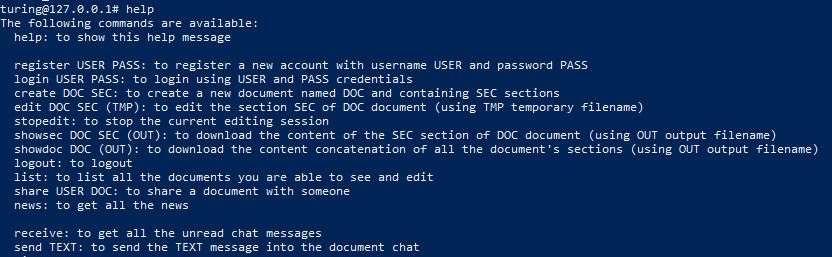
\includegraphics[width=0.8\linewidth]{assets/help_message}
\end{figure}
